\documentclass{standalone}
\usepackage{tikz}
\usetikzlibrary{patterns, positioning}

\begin{document}
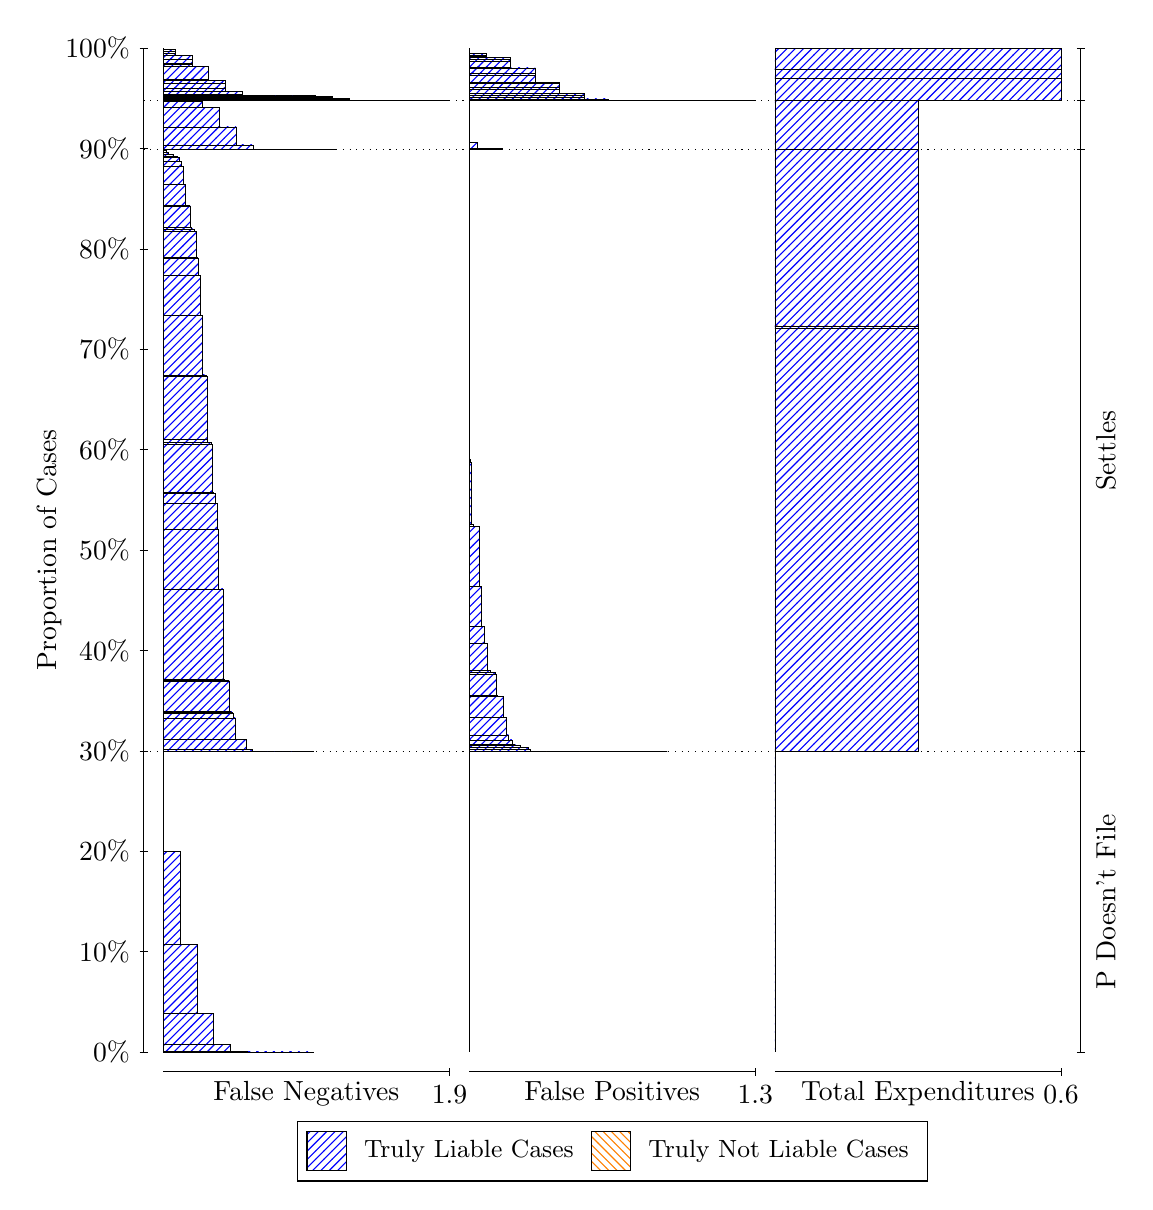
\begin{tikzpicture}
\draw[black, very thin] (1.5,1.75) -- (1.5,14.5);
\node[rotate=90, anchor=center] at (0.3, 8.125) {Proportion of Cases};
\draw[black, very thin] (1.45,1.75) -- (1.55,1.75);
\node[anchor=east] at (1.45, 1.75) {0\%};
\draw[black, very thin] (1.45,3.025) -- (1.55,3.025);
\node[anchor=east] at (1.45, 3.025) {10\%};
\draw[black, very thin] (1.45,4.3) -- (1.55,4.3);
\node[anchor=east] at (1.45, 4.3) {20\%};
\draw[black, very thin] (1.45,5.575) -- (1.55,5.575);
\node[anchor=east] at (1.45, 5.575) {30\%};
\draw[black, very thin] (1.45,6.85) -- (1.55,6.85);
\node[anchor=east] at (1.45, 6.85) {40\%};
\draw[black, very thin] (1.45,8.125) -- (1.55,8.125);
\node[anchor=east] at (1.45, 8.125) {50\%};
\draw[black, very thin] (1.45,9.4) -- (1.55,9.4);
\node[anchor=east] at (1.45, 9.4) {60\%};
\draw[black, very thin] (1.45,10.675) -- (1.55,10.675);
\node[anchor=east] at (1.45, 10.675) {70\%};
\draw[black, very thin] (1.45,11.95) -- (1.55,11.95);
\node[anchor=east] at (1.45, 11.95) {80\%};
\draw[black, very thin] (1.45,13.225) -- (1.55,13.225);
\node[anchor=east] at (1.45, 13.225) {90\%};
\draw[black, very thin] (1.45,14.5) -- (1.55,14.5);
\node[anchor=east] at (1.45, 14.5) {100\%};

\draw[black, very thin] (13.4,1.75) -- (13.4,14.5);
\draw[black, very thin] (13.35,1.75) -- (13.45,1.75);
\node[anchor=west] at (13.35, 1.75) {};
\draw[black, very thin] (13.35,5.563) -- (13.45,5.563);
\node[anchor=west] at (13.35, 5.563) {};
\draw[black, very thin] (13.35,13.21) -- (13.45,13.21);
\node[anchor=west] at (13.35, 13.21) {};
\draw[black, very thin] (13.35,13.833) -- (13.45,13.833);
\node[anchor=west] at (13.35, 13.833) {};
\draw[black, very thin] (13.35,14.5) -- (13.45,14.5);
\node[anchor=west] at (13.35, 14.5) {};

\draw[black, very thin, pattern color=blue, pattern=north east lines] (1.75,1.75) rectangle (3.6623,1.75);
\draw[black, very thin, pattern color=blue, pattern=north east lines] (1.75,1.75) rectangle (3.4498,1.75);
\draw[black, very thin, pattern color=blue, pattern=north east lines] (1.75,1.75) rectangle (3.2373,1.75);
\draw[black, very thin, pattern color=blue, pattern=north east lines] (1.75,1.75) rectangle (3.0249,1.7503);
\draw[black, very thin, pattern color=blue, pattern=north east lines] (1.75,1.7503) rectangle (2.8124,1.7582);
\draw[black, very thin, pattern color=blue, pattern=north east lines] (1.75,1.7582) rectangle (2.5999,1.8434);
\draw[black, very thin, pattern color=blue, pattern=north east lines] (1.75,1.8434) rectangle (2.3874,2.2366);
\draw[black, very thin, pattern color=blue, pattern=north east lines] (1.75,2.2366) rectangle (2.175,3.1157);
\draw[black, very thin, pattern color=blue, pattern=north east lines] (1.75,3.1157) rectangle (1.9625,4.2995);
\draw[black, very thin, pattern color=orange, pattern=north west lines] (1.75,4.2995) rectangle (1.75,4.2995);
\draw[black, very thin, pattern color=blue, pattern=north east lines] (1.75,4.2995) rectangle (1.75,5.563);
\draw[black, very thin, pattern color=blue, pattern=north east lines] (1.75,5.563) rectangle (3.6623,5.563);
\draw[black, very thin, pattern color=blue, pattern=north east lines] (1.75,5.563) rectangle (3.5667,5.563);
\draw[black, very thin, pattern color=blue, pattern=north east lines] (1.75,5.563) rectangle (3.4711,5.563);
\draw[black, very thin, pattern color=blue, pattern=north east lines] (1.75,5.563) rectangle (3.4498,5.563);
\draw[black, very thin, pattern color=blue, pattern=north east lines] (1.75,5.563) rectangle (3.3754,5.563);
\draw[black, very thin, pattern color=blue, pattern=north east lines] (1.75,5.563) rectangle (3.3542,5.563);
\draw[black, very thin, pattern color=blue, pattern=north east lines] (1.75,5.563) rectangle (3.2798,5.563);
\draw[black, very thin, pattern color=blue, pattern=north east lines] (1.75,5.563) rectangle (3.2586,5.563);
\draw[black, very thin, pattern color=blue, pattern=north east lines] (1.75,5.563) rectangle (3.2373,5.563);
\draw[black, very thin, pattern color=blue, pattern=north east lines] (1.75,5.563) rectangle (3.163,5.563);
\draw[black, very thin, pattern color=blue, pattern=north east lines] (1.75,5.563) rectangle (3.1417,5.563);
\draw[black, very thin, pattern color=blue, pattern=north east lines] (1.75,5.563) rectangle (3.0886,5.5641);
\draw[black, very thin, pattern color=blue, pattern=north east lines] (1.75,5.5641) rectangle (3.0673,5.5641);
\draw[black, very thin, pattern color=blue, pattern=north east lines] (1.75,5.5641) rectangle (3.0461,5.5641);
\draw[black, very thin, pattern color=blue, pattern=north east lines] (1.75,5.5641) rectangle (3.0249,5.5641);
\draw[black, very thin, pattern color=blue, pattern=north east lines] (1.75,5.5641) rectangle (2.993,5.5642);
\draw[black, very thin, pattern color=blue, pattern=north east lines] (1.75,5.5642) rectangle (2.9505,5.5642);
\draw[black, very thin, pattern color=blue, pattern=north east lines] (1.75,5.5642) rectangle (2.9292,5.5642);
\draw[black, very thin, pattern color=blue, pattern=north east lines] (1.75,5.5642) rectangle (2.8761,5.5943);
\draw[black, very thin, pattern color=blue, pattern=north east lines] (1.75,5.5943) rectangle (2.8549,5.5968);
\draw[black, very thin, pattern color=blue, pattern=north east lines] (1.75,5.5968) rectangle (2.8336,5.5972);
\draw[black, very thin, pattern color=blue, pattern=north east lines] (1.75,5.5972) rectangle (2.8124,5.5974);
\draw[black, very thin, pattern color=blue, pattern=north east lines] (1.75,5.5974) rectangle (2.8018,5.7195);
\draw[black, very thin, pattern color=blue, pattern=north east lines] (1.75,5.7195) rectangle (2.7805,5.7197);
\draw[black, very thin, pattern color=blue, pattern=north east lines] (1.75,5.7197) rectangle (2.738,5.7206);
\draw[black, very thin, pattern color=blue, pattern=north east lines] (1.75,5.7206) rectangle (2.7168,5.7213);
\draw[black, very thin, pattern color=blue, pattern=north east lines] (1.75,5.7213) rectangle (2.6636,5.994);
\draw[black, very thin, pattern color=blue, pattern=north east lines] (1.75,5.994) rectangle (2.6424,6.0513);
\draw[black, very thin, pattern color=blue, pattern=north east lines] (1.75,6.0513) rectangle (2.6212,6.0688);
\draw[black, very thin, pattern color=blue, pattern=north east lines] (1.75,6.0688) rectangle (2.5999,6.0726);
\draw[black, very thin, pattern color=blue, pattern=north east lines] (1.75,6.0726) rectangle (2.5893,6.4637);
\draw[black, very thin, pattern color=blue, pattern=north east lines] (1.75,6.4637) rectangle (2.568,6.4691);
\draw[black, very thin, pattern color=blue, pattern=north east lines] (1.75,6.4691) rectangle (2.5255,6.4806);
\draw[black, very thin, pattern color=blue, pattern=north east lines] (1.75,6.4806) rectangle (2.5149,7.6221);
\draw[black, very thin, pattern color=blue, pattern=north east lines] (1.75,7.6221) rectangle (2.5043,7.632);
\draw[black, very thin, pattern color=blue, pattern=north east lines] (1.75,7.632) rectangle (2.4512,8.3897);
\draw[black, very thin, pattern color=blue, pattern=north east lines] (1.75,8.3897) rectangle (2.4299,8.7122);
\draw[black, very thin, pattern color=blue, pattern=north east lines] (1.75,8.7122) rectangle (2.4087,8.8512);
\draw[black, very thin, pattern color=blue, pattern=north east lines] (1.75,8.8512) rectangle (2.3874,8.8643);
\draw[black, very thin, pattern color=blue, pattern=north east lines] (1.75,8.8643) rectangle (2.3768,9.4705);
\draw[black, very thin, pattern color=blue, pattern=north east lines] (1.75,9.4705) rectangle (2.3556,9.4963);
\draw[black, very thin, pattern color=blue, pattern=north east lines] (1.75,9.4963) rectangle (2.3131,9.5326);
\draw[black, very thin, pattern color=blue, pattern=north east lines] (1.75,9.5326) rectangle (2.3024,10.325);
\draw[black, very thin, pattern color=blue, pattern=north east lines] (1.75,10.325) rectangle (2.2918,10.35);
\draw[black, very thin, pattern color=blue, pattern=north east lines] (1.75,10.35) rectangle (2.2387,11.108);
\draw[black, very thin, pattern color=blue, pattern=north east lines] (1.75,11.108) rectangle (2.2174,11.617);
\draw[black, very thin, pattern color=blue, pattern=north east lines] (1.75,11.617) rectangle (2.1962,11.828);
\draw[black, very thin, pattern color=blue, pattern=north east lines] (1.75,11.828) rectangle (2.175,11.837);
\draw[black, very thin, pattern color=blue, pattern=north east lines] (1.75,11.837) rectangle (2.1643,12.178);
\draw[black, very thin, pattern color=blue, pattern=north east lines] (1.75,12.178) rectangle (2.1431,12.203);
\draw[black, very thin, pattern color=blue, pattern=north east lines] (1.75,12.203) rectangle (2.1006,12.229);
\draw[black, very thin, pattern color=blue, pattern=north east lines] (1.75,12.229) rectangle (2.09,12.496);
\draw[black, very thin, pattern color=blue, pattern=north east lines] (1.75,12.496) rectangle (2.0793,12.506);
\draw[black, very thin, pattern color=blue, pattern=north east lines] (1.75,12.506) rectangle (2.0262,12.776);
\draw[black, very thin, pattern color=blue, pattern=north east lines] (1.75,12.776) rectangle (2.005,12.995);
\draw[black, very thin, pattern color=blue, pattern=north east lines] (1.75,12.995) rectangle (1.9837,13.058);
\draw[black, very thin, pattern color=blue, pattern=north east lines] (1.75,13.058) rectangle (1.9625,13.06);
\draw[black, very thin, pattern color=blue, pattern=north east lines] (1.75,13.06) rectangle (1.9519,13.118);
\draw[black, very thin, pattern color=blue, pattern=north east lines] (1.75,13.118) rectangle (1.9306,13.123);
\draw[black, very thin, pattern color=blue, pattern=north east lines] (1.75,13.123) rectangle (1.8881,13.126);
\draw[black, very thin, pattern color=blue, pattern=north east lines] (1.75,13.126) rectangle (1.8775,13.152);
\draw[black, very thin, pattern color=blue, pattern=north east lines] (1.75,13.152) rectangle (1.8669,13.153);
\draw[black, very thin, pattern color=blue, pattern=north east lines] (1.75,13.153) rectangle (1.8137,13.179);
\draw[black, very thin, pattern color=blue, pattern=north east lines] (1.75,13.179) rectangle (1.7925,13.202);
\draw[black, very thin, pattern color=blue, pattern=north east lines] (1.75,13.202) rectangle (1.7712,13.206);
\draw[black, very thin, pattern color=orange, pattern=north west lines] (1.75,13.206) rectangle (1.75,13.206);
\draw[black, very thin, pattern color=blue, pattern=north east lines] (1.75,13.206) rectangle (1.75,13.21);
\draw[black, very thin, pattern color=blue, pattern=north east lines] (1.75,13.21) rectangle (3.9491,13.21);
\draw[black, very thin, pattern color=blue, pattern=north east lines] (1.75,13.21) rectangle (3.7366,13.21);
\draw[black, very thin, pattern color=blue, pattern=north east lines] (1.75,13.21) rectangle (3.5242,13.21);
\draw[black, very thin, pattern color=blue, pattern=north east lines] (1.75,13.21) rectangle (3.3117,13.21);
\draw[black, very thin, pattern color=blue, pattern=north east lines] (1.75,13.21) rectangle (3.0992,13.214);
\draw[black, very thin, pattern color=blue, pattern=north east lines] (1.75,13.214) rectangle (2.8867,13.271);
\draw[black, very thin, pattern color=blue, pattern=north east lines] (1.75,13.271) rectangle (2.6743,13.498);
\draw[black, very thin, pattern color=blue, pattern=north east lines] (1.75,13.498) rectangle (2.4618,13.742);
\draw[black, very thin, pattern color=blue, pattern=north east lines] (1.75,13.742) rectangle (2.2493,13.822);
\draw[black, very thin, pattern color=blue, pattern=north east lines] (1.75,13.822) rectangle (2.0368,13.833);
\draw[black, very thin, pattern color=orange, pattern=north west lines] (1.75,13.833) rectangle (1.75,13.833);
\draw[black, very thin, pattern color=blue, pattern=north east lines] (1.75,13.833) rectangle (5.3833,13.833);
\draw[black, very thin, pattern color=blue, pattern=north east lines] (1.75,13.833) rectangle (5.1709,13.833);
\draw[black, very thin, pattern color=blue, pattern=north east lines] (1.75,13.833) rectangle (4.9584,13.833);
\draw[black, very thin, pattern color=blue, pattern=north east lines] (1.75,13.833) rectangle (4.7459,13.833);
\draw[black, very thin, pattern color=blue, pattern=north east lines] (1.75,13.833) rectangle (4.7459,13.833);
\draw[black, very thin, pattern color=blue, pattern=north east lines] (1.75,13.833) rectangle (4.5334,13.834);
\draw[black, very thin, pattern color=blue, pattern=north east lines] (1.75,13.834) rectangle (4.5334,13.834);
\draw[black, very thin, pattern color=blue, pattern=north east lines] (1.75,13.834) rectangle (4.321,13.835);
\draw[black, very thin, pattern color=blue, pattern=north east lines] (1.75,13.835) rectangle (4.321,13.838);
\draw[black, very thin, pattern color=blue, pattern=north east lines] (1.75,13.838) rectangle (4.1085,13.847);
\draw[black, very thin, pattern color=blue, pattern=north east lines] (1.75,13.847) rectangle (4.1085,13.856);
\draw[black, very thin, pattern color=blue, pattern=north east lines] (1.75,13.856) rectangle (4.0235,13.856);
\draw[black, very thin, pattern color=blue, pattern=north east lines] (1.75,13.856) rectangle (3.896,13.877);
\draw[black, very thin, pattern color=blue, pattern=north east lines] (1.75,13.877) rectangle (3.896,13.885);
\draw[black, very thin, pattern color=blue, pattern=north east lines] (1.75,13.885) rectangle (3.811,13.885);
\draw[black, very thin, pattern color=blue, pattern=north east lines] (1.75,13.885) rectangle (3.6835,13.895);
\draw[black, very thin, pattern color=blue, pattern=north east lines] (1.75,13.895) rectangle (3.5985,13.895);
\draw[black, very thin, pattern color=blue, pattern=north east lines] (1.75,13.895) rectangle (3.5985,13.895);
\draw[black, very thin, pattern color=blue, pattern=north east lines] (1.75,13.895) rectangle (3.4711,13.896);
\draw[black, very thin, pattern color=blue, pattern=north east lines] (1.75,13.896) rectangle (3.3861,13.896);
\draw[black, very thin, pattern color=blue, pattern=north east lines] (1.75,13.896) rectangle (3.3861,13.896);
\draw[black, very thin, pattern color=blue, pattern=north east lines] (1.75,13.896) rectangle (3.2586,13.896);
\draw[black, very thin, pattern color=blue, pattern=north east lines] (1.75,13.896) rectangle (3.2586,13.896);
\draw[black, very thin, pattern color=blue, pattern=north east lines] (1.75,13.896) rectangle (3.1736,13.896);
\draw[black, very thin, pattern color=blue, pattern=north east lines] (1.75,13.896) rectangle (3.0461,13.896);
\draw[black, very thin, pattern color=blue, pattern=north east lines] (1.75,13.896) rectangle (3.0461,13.896);
\draw[black, very thin, pattern color=blue, pattern=north east lines] (1.75,13.896) rectangle (2.9611,13.902);
\draw[black, very thin, pattern color=blue, pattern=north east lines] (1.75,13.902) rectangle (2.8336,13.902);
\draw[black, very thin, pattern color=blue, pattern=north east lines] (1.75,13.902) rectangle (2.7486,13.909);
\draw[black, very thin, pattern color=blue, pattern=north east lines] (1.75,13.909) rectangle (2.7486,13.95);
\draw[black, very thin, pattern color=blue, pattern=north east lines] (1.75,13.95) rectangle (2.6212,13.95);
\draw[black, very thin, pattern color=blue, pattern=north east lines] (1.75,13.95) rectangle (2.5362,13.954);
\draw[black, very thin, pattern color=blue, pattern=north east lines] (1.75,13.954) rectangle (2.5362,13.994);
\draw[black, very thin, pattern color=blue, pattern=north east lines] (1.75,13.994) rectangle (2.5362,14.057);
\draw[black, very thin, pattern color=blue, pattern=north east lines] (1.75,14.057) rectangle (2.5362,14.086);
\draw[black, very thin, pattern color=blue, pattern=north east lines] (1.75,14.086) rectangle (2.3237,14.109);
\draw[black, very thin, pattern color=blue, pattern=north east lines] (1.75,14.109) rectangle (2.3237,14.267);
\draw[black, very thin, pattern color=blue, pattern=north east lines] (1.75,14.267) rectangle (2.1112,14.294);
\draw[black, very thin, pattern color=blue, pattern=north east lines] (1.75,14.294) rectangle (2.1112,14.309);
\draw[black, very thin, pattern color=blue, pattern=north east lines] (1.75,14.309) rectangle (2.1112,14.363);
\draw[black, very thin, pattern color=blue, pattern=north east lines] (1.75,14.363) rectangle (2.1112,14.411);
\draw[black, very thin, pattern color=blue, pattern=north east lines] (1.75,14.411) rectangle (1.8987,14.432);
\draw[black, very thin, pattern color=blue, pattern=north east lines] (1.75,14.432) rectangle (1.8987,14.463);
\draw[black, very thin, pattern color=blue, pattern=north east lines] (1.75,14.463) rectangle (1.8987,14.478);
\draw[black, very thin, pattern color=orange, pattern=north west lines] (1.75,14.478) rectangle (1.75,14.478);
\draw[black, very thin, pattern color=blue, pattern=north east lines] (1.75,14.478) rectangle (1.75,14.5);
\draw[black, very thin, pattern color=orange, pattern=north west lines] (5.6333,1.75) rectangle (5.6333,1.75);
\draw[black, very thin, pattern color=blue, pattern=north east lines] (5.6333,1.75) rectangle (5.6333,5.563);
\draw[black, very thin, pattern color=orange, pattern=north west lines] (5.6333,5.563) rectangle (8.1487,5.563);
\draw[black, very thin, pattern color=blue, pattern=north east lines] (5.6333,5.563) rectangle (8.1487,5.563);
\draw[black, very thin, pattern color=blue, pattern=north east lines] (5.6333,5.563) rectangle (7.8382,5.563);
\draw[black, very thin, pattern color=orange, pattern=north west lines] (5.6333,5.563) rectangle (7.7295,5.563);
\draw[black, very thin, pattern color=blue, pattern=north east lines] (5.6333,5.563) rectangle (7.7295,5.563);
\draw[black, very thin, pattern color=blue, pattern=north east lines] (5.6333,5.563) rectangle (7.5276,5.563);
\draw[black, very thin, pattern color=orange, pattern=north west lines] (5.6333,5.563) rectangle (7.45,5.563);
\draw[black, very thin, pattern color=blue, pattern=north east lines] (5.6333,5.563) rectangle (7.45,5.563);
\draw[black, very thin, pattern color=blue, pattern=north east lines] (5.6333,5.563) rectangle (7.4189,5.563);
\draw[black, very thin, pattern color=orange, pattern=north west lines] (5.6333,5.563) rectangle (7.3103,5.563);
\draw[black, very thin, pattern color=blue, pattern=north east lines] (5.6333,5.563) rectangle (7.3103,5.563);
\draw[black, very thin, pattern color=blue, pattern=north east lines] (5.6333,5.563) rectangle (7.2171,5.563);
\draw[black, very thin, pattern color=blue, pattern=north east lines] (5.6333,5.563) rectangle (7.1395,5.563);
\draw[black, very thin, pattern color=blue, pattern=north east lines] (5.6333,5.563) rectangle (7.1084,5.563);
\draw[black, very thin, pattern color=orange, pattern=north west lines] (5.6333,5.563) rectangle (7.0308,5.563);
\draw[black, very thin, pattern color=blue, pattern=north east lines] (5.6333,5.563) rectangle (7.0308,5.563);
\draw[black, very thin, pattern color=blue, pattern=north east lines] (5.6333,5.563) rectangle (6.9997,5.563);
\draw[black, very thin, pattern color=blue, pattern=north east lines] (5.6333,5.563) rectangle (6.9066,5.563);
\draw[black, very thin, pattern color=orange, pattern=north west lines] (5.6333,5.563) rectangle (6.891,5.563);
\draw[black, very thin, pattern color=blue, pattern=north east lines] (5.6333,5.563) rectangle (6.891,5.563);
\draw[black, very thin, pattern color=blue, pattern=north east lines] (5.6333,5.563) rectangle (6.8289,5.563);
\draw[black, very thin, pattern color=blue, pattern=north east lines] (5.6333,5.563) rectangle (6.7979,5.563);
\draw[black, very thin, pattern color=orange, pattern=north west lines] (5.6333,5.563) rectangle (6.7513,5.563);
\draw[black, very thin, pattern color=blue, pattern=north east lines] (5.6333,5.563) rectangle (6.7513,5.5631);
\draw[black, very thin, pattern color=blue, pattern=north east lines] (5.6333,5.5631) rectangle (6.7202,5.5636);
\draw[black, very thin, pattern color=blue, pattern=north east lines] (5.6333,5.5636) rectangle (6.6892,5.5642);
\draw[black, very thin, pattern color=orange, pattern=north west lines] (5.6333,5.5642) rectangle (6.6115,5.5642);
\draw[black, very thin, pattern color=blue, pattern=north east lines] (5.6333,5.5642) rectangle (6.6115,5.5642);
\draw[black, very thin, pattern color=blue, pattern=north east lines] (5.6333,5.5642) rectangle (6.596,5.5647);
\draw[black, very thin, pattern color=blue, pattern=north east lines] (5.6333,5.5647) rectangle (6.5805,5.5648);
\draw[black, very thin, pattern color=blue, pattern=north east lines] (5.6333,5.5648) rectangle (6.5184,5.565);
\draw[black, very thin, pattern color=blue, pattern=north east lines] (5.6333,5.565) rectangle (6.4873,5.5674);
\draw[black, very thin, pattern color=orange, pattern=north west lines] (5.6333,5.5674) rectangle (6.4718,5.5674);
\draw[black, very thin, pattern color=blue, pattern=north east lines] (5.6333,5.5674) rectangle (6.4718,5.5674);
\draw[black, very thin, pattern color=blue, pattern=north east lines] (5.6333,5.5674) rectangle (6.4407,5.5713);
\draw[black, very thin, pattern color=blue, pattern=north east lines] (5.6333,5.5713) rectangle (6.4097,5.5938);
\draw[black, very thin, pattern color=blue, pattern=north east lines] (5.6333,5.5938) rectangle (6.3786,5.6201);
\draw[black, very thin, pattern color=blue, pattern=north east lines] (5.6333,5.6201) rectangle (6.301,5.6208);
\draw[black, very thin, pattern color=blue, pattern=north east lines] (5.6333,5.6208) rectangle (6.2855,5.647);
\draw[black, very thin, pattern color=blue, pattern=north east lines] (5.6333,5.647) rectangle (6.2699,5.6506);
\draw[black, very thin, pattern color=blue, pattern=north east lines] (5.6333,5.6506) rectangle (6.2078,5.6552);
\draw[black, very thin, pattern color=blue, pattern=north east lines] (5.6333,5.6552) rectangle (6.1768,5.7135);
\draw[black, very thin, pattern color=blue, pattern=north east lines] (5.6333,5.7135) rectangle (6.1613,5.7148);
\draw[black, very thin, pattern color=blue, pattern=north east lines] (5.6333,5.7148) rectangle (6.1302,5.7778);
\draw[black, very thin, pattern color=blue, pattern=north east lines] (5.6333,5.7778) rectangle (6.0991,5.9975);
\draw[black, very thin, pattern color=blue, pattern=north east lines] (5.6333,5.9975) rectangle (6.0681,6.2672);
\draw[black, very thin, pattern color=blue, pattern=north east lines] (5.6333,6.2672) rectangle (5.9905,6.2773);
\draw[black, very thin, pattern color=blue, pattern=north east lines] (5.6333,6.2773) rectangle (5.9749,6.5447);
\draw[black, very thin, pattern color=blue, pattern=north east lines] (5.6333,6.5447) rectangle (5.9594,6.5706);
\draw[black, very thin, pattern color=blue, pattern=north east lines] (5.6333,6.5706) rectangle (5.8973,6.5954);
\draw[black, very thin, pattern color=blue, pattern=north east lines] (5.6333,6.5954) rectangle (5.8662,6.9362);
\draw[black, very thin, pattern color=blue, pattern=north east lines] (5.6333,6.9362) rectangle (5.8507,6.945);
\draw[black, very thin, pattern color=blue, pattern=north east lines] (5.6333,6.945) rectangle (5.8197,7.1561);
\draw[black, very thin, pattern color=blue, pattern=north east lines] (5.6333,7.1561) rectangle (5.7886,7.6656);
\draw[black, very thin, pattern color=blue, pattern=north east lines] (5.6333,7.6656) rectangle (5.7575,8.4235);
\draw[black, very thin, pattern color=blue, pattern=north east lines] (5.6333,8.4235) rectangle (5.6799,8.4483);
\draw[black, very thin, pattern color=blue, pattern=north east lines] (5.6333,8.4483) rectangle (5.6644,9.2407);
\draw[black, very thin, pattern color=blue, pattern=north east lines] (5.6333,9.2407) rectangle (5.6489,9.2769);
\draw[black, very thin, pattern color=blue, pattern=north east lines] (5.6333,9.2769) rectangle (5.6333,13.21);
\draw[black, very thin, pattern color=orange, pattern=north west lines] (5.6333,13.21) rectangle (6.0526,13.21);
\draw[black, very thin, pattern color=blue, pattern=north east lines] (5.6333,13.21) rectangle (6.0526,13.221);
\draw[black, very thin, pattern color=blue, pattern=north east lines] (5.6333,13.221) rectangle (5.742,13.301);
\draw[black, very thin, pattern color=blue, pattern=north east lines] (5.6333,13.301) rectangle (5.6333,13.833);
\draw[black, very thin, pattern color=orange, pattern=north west lines] (5.6333,13.833) rectangle (9.2667,13.833);
\draw[black, very thin, pattern color=blue, pattern=north east lines] (5.6333,13.833) rectangle (9.2667,13.833);
\draw[black, very thin, pattern color=orange, pattern=north west lines] (5.6333,13.833) rectangle (8.9561,13.833);
\draw[black, very thin, pattern color=blue, pattern=north east lines] (5.6333,13.833) rectangle (8.9561,13.833);
\draw[black, very thin, pattern color=blue, pattern=north east lines] (5.6333,13.833) rectangle (8.6456,13.833);
\draw[black, very thin, pattern color=orange, pattern=north west lines] (5.6333,13.833) rectangle (8.6456,13.833);
\draw[black, very thin, pattern color=blue, pattern=north east lines] (5.6333,13.833) rectangle (8.6456,13.833);
\draw[black, very thin, pattern color=blue, pattern=north east lines] (5.6333,13.833) rectangle (8.335,13.833);
\draw[black, very thin, pattern color=blue, pattern=north east lines] (5.6333,13.833) rectangle (8.335,13.833);
\draw[black, very thin, pattern color=orange, pattern=north west lines] (5.6333,13.833) rectangle (8.335,13.833);
\draw[black, very thin, pattern color=blue, pattern=north east lines] (5.6333,13.833) rectangle (8.335,13.833);
\draw[black, very thin, pattern color=orange, pattern=north west lines] (5.6333,13.833) rectangle (8.0245,13.833);
\draw[black, very thin, pattern color=blue, pattern=north east lines] (5.6333,13.833) rectangle (8.0245,13.834);
\draw[black, very thin, pattern color=blue, pattern=north east lines] (5.6333,13.834) rectangle (8.0245,13.834);
\draw[black, very thin, pattern color=blue, pattern=north east lines] (5.6333,13.834) rectangle (8.0245,13.834);
\draw[black, very thin, pattern color=orange, pattern=north west lines] (5.6333,13.834) rectangle (7.714,13.834);
\draw[black, very thin, pattern color=blue, pattern=north east lines] (5.6333,13.834) rectangle (7.714,13.837);
\draw[black, very thin, pattern color=blue, pattern=north east lines] (5.6333,13.837) rectangle (7.714,13.837);
\draw[black, very thin, pattern color=blue, pattern=north east lines] (5.6333,13.837) rectangle (7.4034,13.841);
\draw[black, very thin, pattern color=orange, pattern=north west lines] (5.6333,13.841) rectangle (7.4034,13.841);
\draw[black, very thin, pattern color=blue, pattern=north east lines] (5.6333,13.841) rectangle (7.4034,13.855);
\draw[black, very thin, pattern color=blue, pattern=north east lines] (5.6333,13.855) rectangle (7.0929,13.87);
\draw[black, very thin, pattern color=blue, pattern=north east lines] (5.6333,13.87) rectangle (7.0929,13.897);
\draw[black, very thin, pattern color=orange, pattern=north west lines] (5.6333,13.897) rectangle (7.0929,13.897);
\draw[black, very thin, pattern color=blue, pattern=north east lines] (5.6333,13.897) rectangle (7.0929,13.923);
\draw[black, very thin, pattern color=blue, pattern=north east lines] (5.6333,13.923) rectangle (6.7823,13.971);
\draw[black, very thin, pattern color=blue, pattern=north east lines] (5.6333,13.971) rectangle (6.7823,14);
\draw[black, very thin, pattern color=orange, pattern=north west lines] (5.6333,14) rectangle (6.7823,14);
\draw[black, very thin, pattern color=blue, pattern=north east lines] (5.6333,14) rectangle (6.7823,14.05);
\draw[black, very thin, pattern color=blue, pattern=north east lines] (5.6333,14.05) rectangle (6.7823,14.051);
\draw[black, very thin, pattern color=blue, pattern=north east lines] (5.6333,14.051) rectangle (6.7823,14.066);
\draw[black, very thin, pattern color=blue, pattern=north east lines] (5.6333,14.066) rectangle (6.4718,14.149);
\draw[black, very thin, pattern color=blue, pattern=north east lines] (5.6333,14.149) rectangle (6.4718,14.185);
\draw[black, very thin, pattern color=blue, pattern=north east lines] (5.6333,14.185) rectangle (6.4718,14.247);
\draw[black, very thin, pattern color=blue, pattern=north east lines] (5.6333,14.247) rectangle (6.1613,14.261);
\draw[black, very thin, pattern color=blue, pattern=north east lines] (5.6333,14.261) rectangle (6.1613,14.333);
\draw[black, very thin, pattern color=blue, pattern=north east lines] (5.6333,14.333) rectangle (6.1613,14.356);
\draw[black, very thin, pattern color=blue, pattern=north east lines] (5.6333,14.356) rectangle (6.1613,14.383);
\draw[black, very thin, pattern color=orange, pattern=north west lines] (5.6333,14.383) rectangle (6.037,14.383);
\draw[black, very thin, pattern color=blue, pattern=north east lines] (5.6333,14.383) rectangle (6.037,14.383);
\draw[black, very thin, pattern color=blue, pattern=north east lines] (5.6333,14.383) rectangle (5.8507,14.398);
\draw[black, very thin, pattern color=blue, pattern=north east lines] (5.6333,14.398) rectangle (5.8507,14.405);
\draw[black, very thin, pattern color=blue, pattern=north east lines] (5.6333,14.405) rectangle (5.8507,14.431);
\draw[black, very thin, pattern color=orange, pattern=north west lines] (5.6333,14.431) rectangle (5.7265,14.431);
\draw[black, very thin, pattern color=blue, pattern=north east lines] (5.6333,14.431) rectangle (5.7265,14.431);
\draw[black, very thin, pattern color=orange, pattern=north west lines] (5.6333,14.431) rectangle (5.6333,14.431);
\draw[black, very thin, pattern color=blue, pattern=north east lines] (5.6333,14.431) rectangle (5.6333,14.5);
\draw[black, very thin, pattern color=orange, pattern=north west lines] (9.5167,1.75) rectangle (9.5167,1.75);
\draw[black, very thin, pattern color=blue, pattern=north east lines] (9.5167,1.75) rectangle (9.5167,5.563);
\draw[black, very thin, pattern color=orange, pattern=north west lines] (9.5167,5.563) rectangle (11.333,5.563);
\draw[black, very thin, pattern color=blue, pattern=north east lines] (9.5167,5.563) rectangle (11.333,10.942);
\draw[black, very thin, pattern color=orange, pattern=north west lines] (9.5167,10.942) rectangle (11.333,10.942);
\draw[black, very thin, pattern color=blue, pattern=north east lines] (9.5167,10.942) rectangle (11.333,10.97);
\draw[black, very thin, pattern color=orange, pattern=north west lines] (9.5167,10.97) rectangle (11.333,10.97);
\draw[black, very thin, pattern color=blue, pattern=north east lines] (9.5167,10.97) rectangle (11.333,13.21);
\draw[black, very thin, pattern color=orange, pattern=north west lines] (9.5167,13.21) rectangle (11.333,13.21);
\draw[black, very thin, pattern color=blue, pattern=north east lines] (9.5167,13.21) rectangle (11.333,13.833);
\draw[black, very thin, pattern color=orange, pattern=north west lines] (9.5167,13.833) rectangle (13.15,13.833);
\draw[black, very thin, pattern color=blue, pattern=north east lines] (9.5167,13.833) rectangle (13.15,14.119);
\draw[black, very thin, pattern color=orange, pattern=north west lines] (9.5167,14.119) rectangle (13.15,14.119);
\draw[black, very thin, pattern color=blue, pattern=north east lines] (9.5167,14.119) rectangle (13.15,14.226);
\draw[black, very thin, pattern color=orange, pattern=north west lines] (9.5167,14.226) rectangle (13.15,14.226);
\draw[black, very thin, pattern color=blue, pattern=north east lines] (9.5167,14.226) rectangle (13.15,14.5);
\draw[black, dotted] (1.5,5.563) -- (13.4,5.563);
\draw[black, dotted] (1.5,13.21) -- (13.4,13.21);
\draw[black, dotted] (1.5,13.833) -- (13.4,13.833);
\draw[black, very thin] (1.75,1.5) -- (5.3833,1.5);
\node[anchor=north] at (3.5667, 1.5) {False Negatives};
\draw[black, very thin] (5.3833,1.45) -- (5.3833,1.55);
\node[anchor=north] at (5.3833, 1.45) {1.9};

\draw[black, very thin] (5.6333,1.5) -- (9.2667,1.5);
\node[anchor=north] at (7.45, 1.5) {False Positives};
\draw[black, very thin] (9.2667,1.45) -- (9.2667,1.55);
\node[anchor=north] at (9.2667, 1.45) {1.3};

\draw[black, very thin] (9.5167,1.5) -- (13.15,1.5);
\node[anchor=north] at (11.333, 1.5) {Total Expenditures};
\draw[black, very thin] (13.15,1.45) -- (13.15,1.55);
\node[anchor=north] at (13.15, 1.45) {0.6};

\node[black, centered, rotate=90] at (13.72, 3.6565) {P Doesn't File};
\node[black, centered, rotate=90] at (13.72, 9.3866) {Settles};



\draw (7.449999999999999,1.5) node[draw=none] (baseCoordinate) {};
\begin{scope}[align=center]
        \matrix[scale=0.5, draw=black, below=0.5cm of baseCoordinate, nodes={draw}, column sep=0.1cm]{
            \node[rectangle, draw, minimum width=0.5cm, minimum height=0.5cm, pattern=north east lines, pattern color=blue] {}; &
            \node[draw=none, font=\small] (B) {Truly Liable Cases}; &
            \node[rectangle, draw, minimum width=0.5cm, minimum height=0.5cm, pattern=north west lines, pattern color=orange] {}; &
            \node[draw=none, font=\small] (B) {Truly Not Liable Cases}; \\
            };
\end{scope}

\end{tikzpicture}
\end{document}